\chapter{Estudio del Problema}

\section{Historia de Re-Volt}
Re-Volt America, en su expresión más simple, es una comunidad de jugadores del videojuego Re-Volt, el cual fue lanzado originalmente en el año 1999 por Acclaim Studios en Londres. Re-Volt es un videojuego de carreras y simulador arcade de autos a control remoto, el cual explora una premisa en donde dichos autos compiten en carreras de radio control en ambientes como museos, supermercados, barcos, sitios de construcción, entre otros. Esto combinado con una mecánica de objetos que pueden ser recogidos por dichos autos para atacar a los competidores, obtener más velocidad, entre otras ventajas.

El arte original de la caratula del juego puede ser apreciado en la figura FIGNUM.


\includegraphics{img/re-volt.jpg}

El primero de septiembre del año 2004, Acclaim Studios se declara en banca rota, y cesa permanentemente todo el desarrollo y mantenimiento que en algún momento proveyó a Re-Volt y a su comunidad. Este suceso, a lo largo de los años, dio lugar a muchas comunidades segmentadas del juego en el internet de ese entonces. Con el tiempo, nuevos sitios y proyectos comenzaron a surgir, tales como el portal web de Re-Volt Race, una página de Re-Volt que se dedicaba a organizar partidas online y mantener tablas de resultados para los jugadores, o Re-Volt: OpenGL (RVGL), una re-escritura moderna del Re-Volt original que todos conocían, ahora disponible para plataformas modernas y otros sistemas operativos además de Windows, como Linux, MacOS, e incluso una versión para dispositivos Android.

Dentro de lo anteriormente enmarcado, aparece en el año 2015 la comunidad de Re-Volt I/O, cuyo logotipo se puede apreciar en la figura FIGNUM. Esta comunidad estaba formada por un grupo de jugadores de Re-Volt, principalmente europeos, quienes incursionaron por primera vez en intentar crear una plataforma estable para el videojuego y su comunidad de jugadores. Este sería un lugar en donde cualquiera que quisiera disfrutar del juego podría encontrar guías de ayuda, tutoriales, descargas y demás contenido para poder instalar y jugar Re-Volt en su computador o dispositivo móvil.


\includegraphics{img/io.png}

En sus inicios, Re-Volt I/O adoptó a RVGL como la distribución estándar de Re-Volt que ofrecería a sus jugadores, haciéndole ganar público y reconocimiento al proyecto publicando enlaces de descarga directos en su página web (re-volt.io), además de entregar soporte y mantener hilos de discusión relacionados con RVGL y sus actualizaciones en su foro oficial (forum.re-volt.io).

En adición a lo anterior, RVGL no era tan sólo una versión modernizada del Re-Volt original, sino que también traía consigo el aspecto más importante que tiene Re-Volt en la actualidad, y el cual mantiene unida y activa a su comunidad en general: el modo multijugador u online. Dicho modo no sólo permitía a los jugadores correr carreras en línea, sino que, además, extendía soporte para que miembros de la comunidad pudiesen diseñar sus propios autos y pistas de manera personalizada, agrandando así, de manera casi infinita, el repertorio de contenido descargable para Re-Volt.

Re-Volt I/O adoptó un sistema en donde su administración elige ciertos autos y pistas hechos por la comunidad cada ciertos meses. De esta forma, todos estos autos y pistas, elegidos a votación, terminan juntos en un paquete de contenido de extensión para RVGL, el cual Re-Volt I/O se encarga de distribuir para que sus usuarios lo descarguen y puedan jugar en línea. De manera habitual, tener este paquete de contenido es obligatorio para poder jugar en las sesiones multijugador organizadas por Re-Volt I/O, lo cual lo convertiría en un estándar para los jugadores que quisieran incorporarse a la comunidad en toda su extensión.

Fue así como Re-Volt I/O, entre finales del 2015 y mediados del 2017, logró consolidarse y llegar a más jugadores que nunca, formando una comunidad activa de amantes del juego quienes, espontáneamente, se reunían a jugar en línea durante la semana utilizando un paquete de contenido adicional para RVGL, el cual todos debían descargar e instalar por separado para poder jugar. Eventualmente, estas partidas en línea adquirieron un horario definido con fechas y horas acordadas con antelación, para así facilitar la asistencia de los jugadores a los eventos de carreras.

En la actualidad, Re-Volt I/O sigue siendo la comunidad de Re-Volt más grande en términos de jugadores y escala, pero en si todas las comunidades de Re-Volt están unidas y se ayudan unas con otras. Después de todo, se trata de un juego nicho, en donde todos intentan hacerlo accesible y fácil de entender para quienes deseen formar parte de su comunidad.

\section{Re-Volt America}
Si bien Re-Volt I/O fue, durante muchos años, la única comunidad grande de Re-Volt a nivel mundial, no fue mucho después de su gran auge que comenzarían a formarse los demás grupos que, a día de hoy, tienen gran relevancia en la escena multijugador de Re-Volt y que, además, cuentan con un numeroso público y gran actividad. Dentro de estas nuevas comunidades se encuentra Re-Volt America, la comunidad de Re-Volt que abarca a todos los jugadores del continente americano, especialmente de latinoamérica. El logotipo oficial de Re-Volt America, o RVA para abreviar, puede apreciarse en la figura FIGNUM.


\includegraphics[width=10cm, height=10cm]{img/rva.png}

La comunidad de Re-Volt America es concebida originalmente en el año 2017, bajo el nombre de Re-Volt Tournament. No fue hasta después de un par de años que esta sería renombrada a Re-Volt America, debido a la procedencia de sus jugadores, la cual era tanto de norte america como de sudamerica.

En el presente año 2023, Re-Volt America cuenta con una gran cantidad de jugadores activos, y con un sistema de puntuación único en la escena de Re-Volt y sus comunidades en línea. Este complejo sistema de puntuación, y su funcionamiento sostenido durante los últimos 6 años, son la base del problema que busca solucionar este proyecto de título. Con el pasar del tiempo, este sistema se ha convertido en algo muy difícil de mantener para los administradores de la comunidad, tanto a nivel logístico como técnico.

A continuación, se presentaría el contexto del problema en detalle.

\section{Contexto del Problema}
Como ya se mencionó anteriormente, Re-Volt es un videojuego de carreras el cual, gracias al surgimiento de RVGL y sus comunidades impulsoras, es jugado mayoritariamente en línea. Pero, ¿a qué nos referimos con ''jugar en línea''?. Para poder entender este concepto, tenemos que ir a lo que es una carrera en términos conceptuales, y las implicaciones que estas conllevan dentro de un contexto competitivo.

Para poder jugar en línea, cada jugador debe elegir un nombre de usuario, el cual puede incluso variar de partida en partida. Esto se hace una vez que ingresa al juego y avanza en el menú hasta llegar al selector de nombre de usuario en forma de neumático. El nombre que el jugador ingrese aquí será el nombre de usuario con el que se identificará a la hora de ser ingresado a los resultados de cada carrera en la que participe. El selector de nombre de usuario se puede apreciar a continuación en la figura FIGNUM.


\includegraphics[width=15cm, height=8cm]{img/username.png}

Las siguientes dos ilustraciones presentan las instancias clave dentro del juego. En la ilustración FIGNUM, se puede apreciar la perspectiva del jugador al momento de jugar Re-Volt. Luego, en la ilustración FIGNUM, se puede ver la tabla de resultados que se muestra por pantalla a medida que los corredores finalizan la carrera.

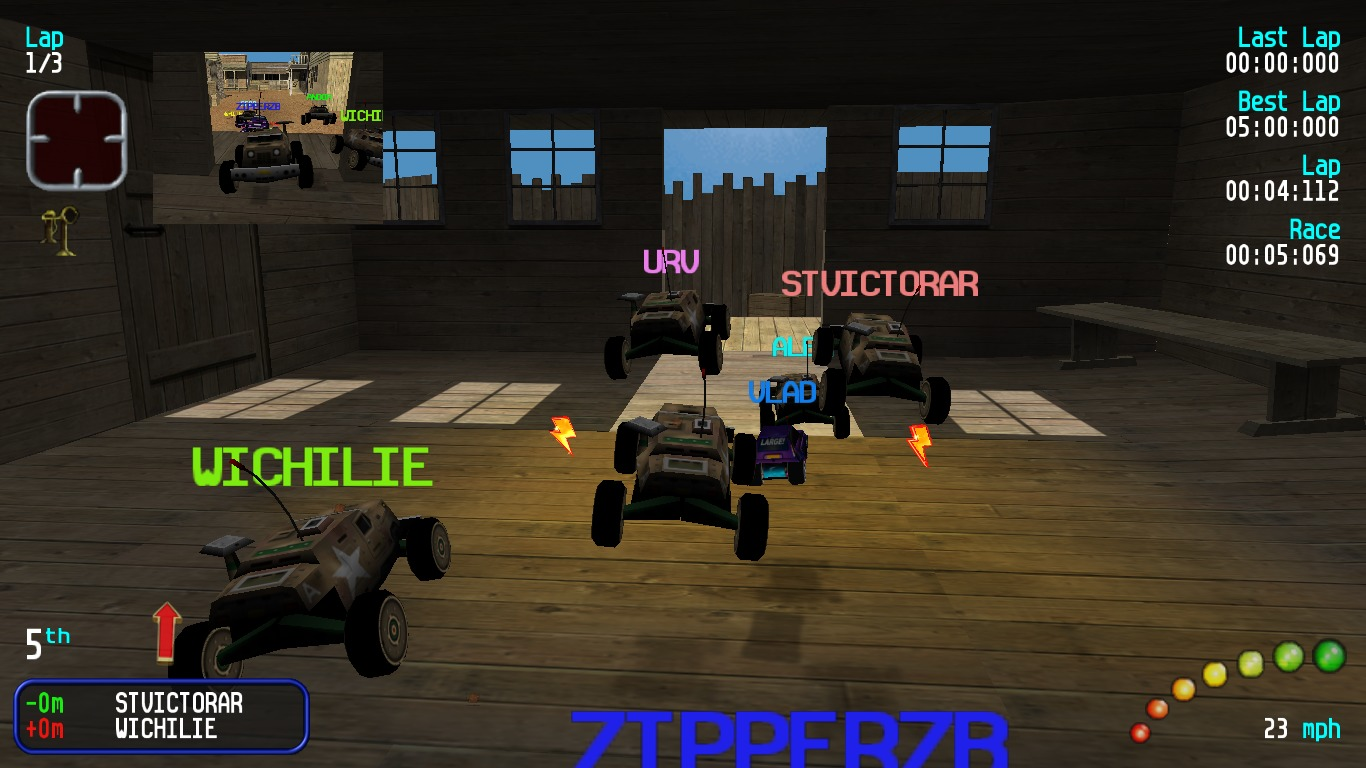
\includegraphics[width=15cm, height=8cm]{img/gameplay.jpg}

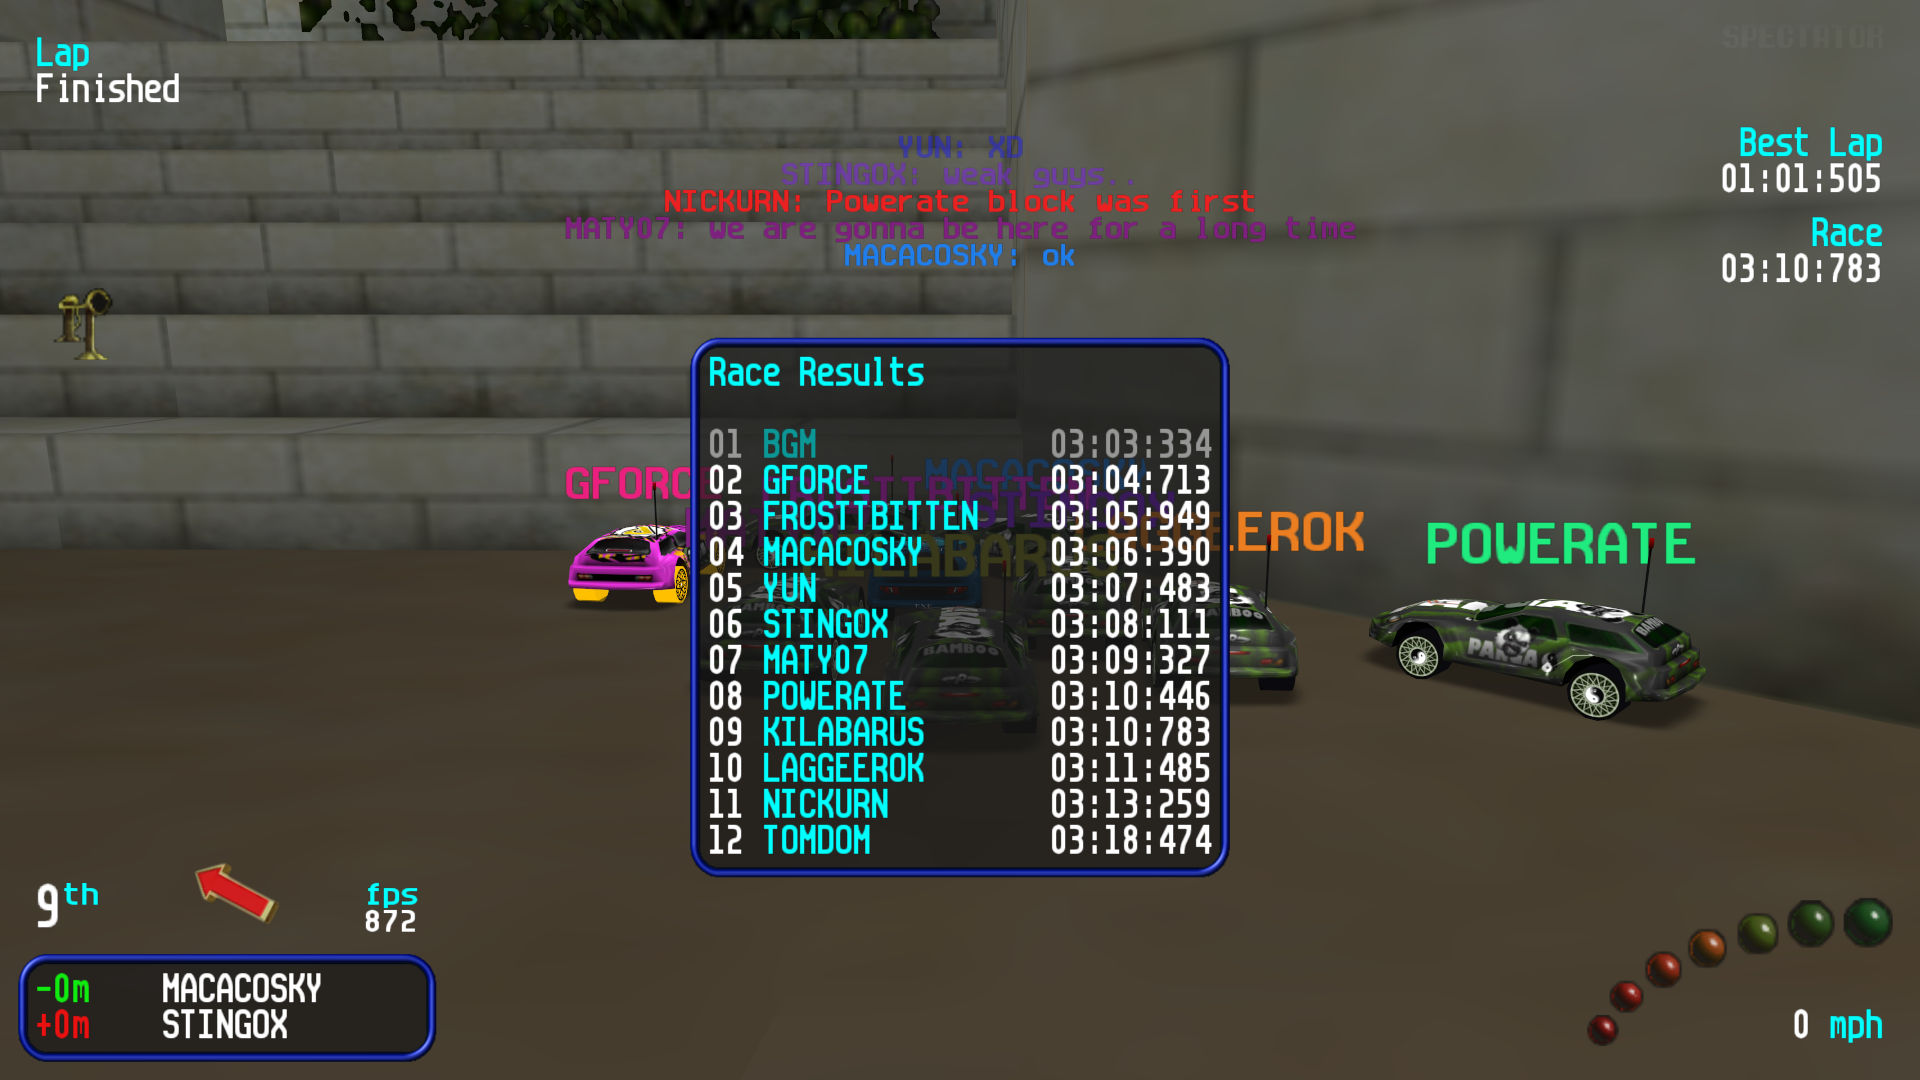
\includegraphics[width=15cm, height=8cm]{img/results.png}

Normalmente, en las partidas en línea, suelen jugarse muchas carreras de manera consecutiva. A estas partidas multijugador se les conoce como ''sesiones''. Cada sesión de Re-Volt consiste en una serie de carreras en pistas determinadas, con cierta clase de autos. Estas determinaciones las realiza el anfitrión de la partida, quien las comunica públicamente de manera oportuna para que todos aquellos que deseen participar las tengan en consideración antes de conectarse a jugar.

Históricamente, Re-Volt America se ha dedicado a organizar sesiones multijugador de Re-Volt para su público, así como también se ha preocupado de llevar la cuenta de los resultados de cada carrera que se ha jugado en ellas mediante un sistema de temporadas. Todos los jugadores que, en algún momento u otro, han participado en las sesiones online organizadas por Re-Volt America, han sido indexados en la base de datos de jugadores que mantiene la comunidad. De esta forma, sus victorias, puntos y otras estadísticas asociadas han sido preservadas a lo largo del tiempo.

Re-Volt America cuenta con un sistema interno para organizar sus sesiones de carreras online, el cual consiste en dividir dichas sesiones en rankings, y estos rankings por temporadas: En un año se celebran dos temporadas. Cada temporada está compuesta de 6 rankings, y cada ranking de 28 sesiones online en total.

Este proyecto se enmarca directamente en este ámbito competitivo que busca generar Re-Volt America para sus usuarios, para poder lograr una mejora sustancial y un cambio revolucionario en la manera en que se llevan estos registros históricos de resultados y como es manejada y procesada la información que se obtiene de dichas sesiones online.

\section{Definiciones, Siglas y Abreviaciones}
A continuación, se definirán algunos conceptos relevantes en el contexto del videojuego Re-Volt y la comunidad de Re-Volt America:

•	Re-Volt: El videojuego Re-Volt, 1999 (https://en.wikipedia.org/wiki/Re-Volt).

•	RV: Re-Volt.

•	RVGL: Re-Volt OpenGL. La reescritura del juego original que es usada por todos los jugadores hoy en día. (https://rvgl.org).

•	Re-Volt I/O: Comunidad Europea de Re-Volt.

•	RVA: Re-Volt America.

•	RTT: Re-Volt Tournament.

•	Sesión: Evento de carreras online del videojuego Re-Volt, en donde dos o más personas compiten en una o más carreras multijugador.

•	Session Log: Archivo separado por comas que contiene un registro crudo de los resultados de las carreras jugadas en una sesión de RVGL.

\section{Problemática Actual}
Desde hace aproximadamente 5 años, Re-Volt America ha mantenido los registros históricos de las sesiones celebradas a diario de manera interna y, a partir de estos registros, se ha mantenido publicando los resultados por sesión y rankings acumulados para todos los jugadores de la comunidad. Además de esto, RVA también se ha encargado hasta la fecha de recoger otro tipo de estadísticas e información de sus jugadores como pueden ser el país, total de puntos acumulados por temporada, carreras corridas, porcentaje por participación y puntajes totales dentro del sistema de puntuación de RVA.

En RVGL, cada carrera consiste en que los jugadores corren en una pista, y al final cada uno termina en una posición dependiendo de quien llega primero a la meta, como en cualquier juego de carreras tradicional. Cada sesión organizada por RVA consiste en 20 carreras que se juegan en 20 pistas diferentes, por lo que en una sesión se producen 20 sets de resultados de carreras. RVGL permite a los jugadores obtener un registro escrito de los resultados de cada carrera jugada en multijugador, escribiendo dichos registros a un archivo separado por comas conocido como “Session Log” por la comunidad. Este es el archivo que utilizan los organizadores de RVA para calcular los resultados oficiales para su eventual publicación.
El sistema interno de RVA asigna un puntaje por posición final de cada jugador en una carrera de la siguiente forma:

Ilustración 3: Puntajes por posición en RVA.
Dichos puntajes, al final de cada sesión, son sumados para obtener un total, normalizados y sometidos a diferentes procesos como la división por posición promedio, multiplicación por porcentaje de participación, entre otras operaciones que ayudan a determinar los resultados finales en el formato de RVA. Dichos resultados cuales terminan viéndose como se muestra en la ilustración 4.

Ilustración 4: Tabla de resultados de RVA.
Todo este proceso de cálculo de resultados es llevado a cabo actualmente de manera semiautomática por los organizadores y administradores de RVA. Este proceso consiste en los siguientes pasos:
1.	Llevar a cabo la sesión multijugador y obtener el Session Log con los resultados crudos de cada carrera.
2.	Pasar dicho Session Log por un programa de escritorio que ayuda a calcular los resultados en el formato de RVA.
3.	Con dicho programa de escritorio, exportar los resultados en un formato separado por comas (archivo CSV).
4.	Tomar los resultados exportados y copiarlos manualmente a un documento maestro en Microsoft Excel, en donde los resultados son indexados junto con el resto.
5.	Agregar cierta información de manera manual, como la fecha de la sesión, número de sesión y corregir nombres de jugadores inválidos.
6.	Publicar una fotografía de los resultados traspasados al documento maestro, y otra foto del ranking total de la temporada que también se mantiene actualizado dentro del mismo documento.
A raíz de este largo y tedioso proceso de cálculo y manejo de resultados es que se ha dado origen a este proyecto, como una oportunidad de mejorar dicho proceso, y poder ofrecer así una mejor experiencia de usuario tanto a los jugadores de RVA, como a los organizadores de la comunidad que dedican su tiempo y pasión por este juego a mantener estos registros históricos al día para todos.

\subsection{Diagrama de la Situación en la Actualidad}
Diagrama en UML

\section{Propuesta de solución}
Debe explicar en términos generales cómo las TIC pueden resolver o mejorar la(s) problemática identificada y quienes serán los usuarios principales, que tecnología se utilizaría para dar soporte a la propuesta.

\section{Soluciones similares disponibles}
Se presentan soluciones similares...

\subsection{Aplicación para Cálculo de Puntos de Re-Volt I/O}
Existe un trabajo similar hace varios años, el cual fue desarrollado por la comunidad europea de RVGL: Re-Volt I/O. Este trabajo es también una aplicación web que permite a los jugadores importar los resultados de las sesiones multijugador y poder visualizarlos dentro de la misma página; sin embargo, dicho proyecto no cuenta con ningún tipo de interconexión entre resultados, lo que quiere decir que cada sesión de carreras publicada en dicho sitio es independiente de otras, por lo cual este proyecto no cuenta con perfiles de usuario, y por ende no permite visualizar estadísticas de ningún tipo, tampoco relacionar tablas de resultados entre sí, y en general fue hecho para ser algo simple y rápido que sirviera para calcular y renderizar resultados de manera oportuna, y no con una visión de persistencia en mente. A continuación, en la ilustración 4 puede apreciarse la tabla de resultados generada por la aplicación web de Re-Volt: I/O.

\subsection{Aplicación para Cálculo de Puntos de RVA}
RVA cuenta con una aplicación de escritorio...

\section{Justificación del Problema}
El videojuego de carreras Re-Volt, creado en 1999, cuya caracterización se representa en la ilustración 1, tiene como premisa ser un juego de carreras de autos a control remoto, los cuales compiten en entornos cotidianos como supermercados, barcos, sitios de construcción, museos, entre otros.
Unos años después de su lanzamiento original, la empresa creadora del juego “Acclaim Studios” quebró, y la base de código del juego fue liberada al público. A partir de esta base el juego fue reescrito completamente y portado a la librería de OpenGL, creándose así Re-Volt: OpenGL o RVGL de manera abreviada.

Re-Volt America, o RVA para abreviar, reúne a los jugadores y creadores de contenido de RVGL de todas partes de América, quienes mantienen vivo el juego organizando eventos como sesiones y torneos multijugador.

Actualmente no existe ninguna plataforma que permita a los usuarios registrarse y visualizar resultados y estadísticas de las sesiones multijugador organizadas por la comunidad. Lo anterior significa que cuando se juegan partidas online no es posible obtener de manera automática rankings, estadísticas por vehículo y menos por usuario, ya que no hay forma de vincular de manera definitiva a los jugadores a través de un perfil dentro del juego. Tal como puede verse en la ilustración 2. Es por ello por lo que un usuario de nuestra comunidad no puede saber cuántas carreras o sesiones ha ganado con cierto auto, o en cierta pista, cómo se compara al resto, qué porcentaje de carreras ha perdido, etc.



